\begin{blocksection}
\question Give the environment diagram and console output that result from running the following code.

\begin{lstlisting}
def swap(x, y):
    x, y = y, x
    return print("Swapped!", x, y)

x, y = 60, 1
a = swap(x, y)
swap(a, y)
\end{lstlisting}

\begin{solution}[2in]
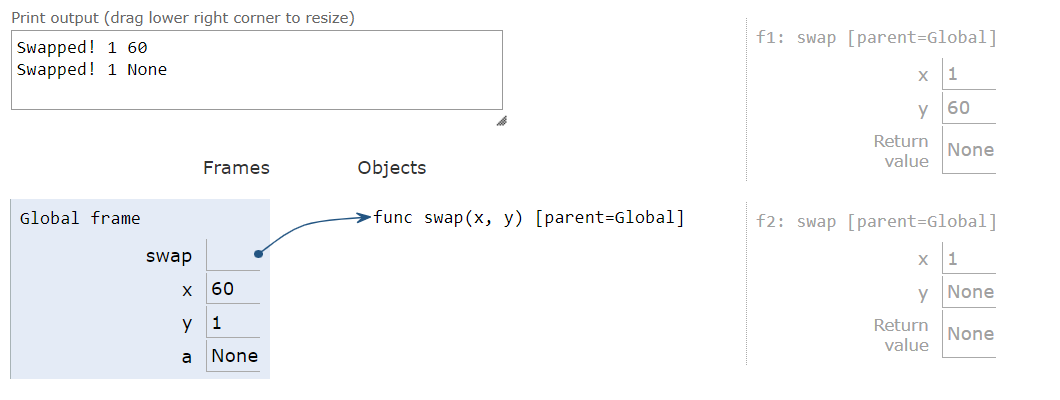
\includegraphics[scale=0.5]{swap.png}
\\
\url{https://tinyurl.com/y68m6qdj}
\end{solution}
\end{blocksection}

\begin{questionmeta}
  This question emphasizes the separation of variables into different scopes. The fact that \lstinline{x} and \lstinline{y} are used in both global and local frames is meant to demonstrate that the same symbol can mean different things in different contexts, and that different frames have domain over their own namespace and---for the most part---cannot change the namespace of other frames. The printed output ("Swapped! ...") and name of the function (\lstinline{swap}) are a bit misleading in this respect because a call to \lstinline{swap(x, y)} will not actually swap the values of \lstinline{x} and \lstinline{y} in the frame where it is called. (That is, \lstinline{x} and \lstinline{y} still have the same values in the global frame after \lstinline{swap} is called on them.) The goal is that students will be surprised/confused by this behavior, and that they will learn from this mental challenge. 

  Some students might have done variable swaps in other languages. If students are confused by this, make sure to explain why same line assignments (eg. \lstinline{x, y = y, x}) work in Python.

  It may also be useful to explain the difference between printing and returning, which can be confusing to some students. 
\end{questionmeta}
